\documentclass[a4paper,11pt,twoside]{article}
\renewcommand{\familydefault}{\sfdefault}      % sans serif font

% -------------------------------------------------
% Packages
% -------------------------------------------------
\usepackage{lmodern}        
\usepackage[T1]{fontenc}
\usepackage[utf8]{inputenc}
\usepackage{pdfpages}      	% For including PDF pages
\usepackage{fancyhdr}      	% For page numbering style
\usepackage{geometry}      	% For page margins
\usepackage{graphicx}      	% For including logos
\usepackage{tocloft}        % For table of contents
\usepackage{hyperref}      	% For clickable table of contents

% -------------------------------------------------
% Page setup
% -------------------------------------------------
% Load current version number
\newcommand{\version}{\input{../../VERSION}}

\renewcommand{\sectionmark}[1]{\markright{\thesection\ #1}}
\renewcommand{\headrulewidth}{0.4pt}
\renewcommand{\footrulewidth}{0pt}

% Set header and footer
\geometry{margin=2.5cm}
\fancyhf{} 				   			% Clear all header and footer fields
\fancyhead[LE, RO]{\thepage}		% Outer edges: page number
\fancyhead[RE]{PCPT}				% Even pages, inner side
\fancyhead[LO]{\rightmark}  		% Odd pages, inner side: section title

% TOC dots for sections
\renewcommand{\cftdotsep}{3}		% Adjust spacing between dots
\renewcommand{\cftsecleader}{\cftdotfill{\cftdotsep}}

% -------------------------------------------------
% Makro for including pdfs 
% -------------------------------------------------
\newcommand{\pdfsection}[3]{%
	\pagestyle{empty}
  	\cleardoublepage
  	\pagestyle{fancy}
  	\includepdf[pages=-,pagecommand=\thispagestyle{fancy},addtotoc={1,section,1,#1,#2}]{#3}%
}

% -------------------------------------------------
% Document
% -------------------------------------------------
\begin{document}

% ---------------- Title Page ----------------
\begin{titlepage}
\thispagestyle{empty}

%\newgeometry{top=4cm,bottom=1.5cm,inner=3cm,outer=2cm}

% ---------------- Header ----------------

\begin{center}
	\vspace*{-2cm}
	\begin{center}
		\Large{\textbf{Friedrich-Alexander-Universit\"at Erlangen-N\"urnberg}} \\[0.5cm]
		
\includegraphics[width=8.5cm]{figures/Logo_FAU.pdf}
	\end{center}
	\noindent\rule{\textwidth}{1pt}
\end{center}

% ---------------- Content ----------------

\vfill

%\begin{center}
	\fontsize{16pt}{0pt}\selectfont\noindent 
	Meinard Müller, Sebastian Strahl 

	\vspace{1.5cm}
	\fontsize{25pt}{0pt}\selectfont\noindent 
	\textbf{PCPT:} A \textbf{P}reparation \textbf{C}ourse in \textbf{P}y\textbf{T}orch

	\vspace{0.5cm}
	\fontsize{16pt}{0pt}\selectfont\noindent 
	Through the Principles of Signal Processing

	\vspace{1.5cm}
	\fontsize{16pt}{0pt}\selectfont\noindent 
	\today \\[1ex] Version \version

	\vspace{2cm}
	\centering
	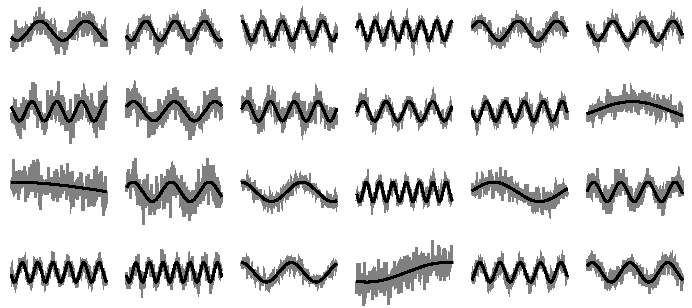
\includegraphics[width=0.8\textwidth]{figures/PCPT_Teaser_bw.pdf}
%\end{center}

\vfill

% ---------------- Footer ----------------

\noindent\rule{\textwidth}{1pt}
\vspace{-0.8cm}
\normalsize
	
\begin{center}
	\begin{minipage}[t]{2.6cm}
	\vspace{0pt}
		
\includegraphics[width=2.5cm]{figures/Logo_AudioLabs.pdf}
	\end{minipage}
	\hfill
	%
	\begin{minipage}[t]{8.5cm}
	\vspace{0pt}
	\centering
	International Audio Laboratories Erlangen\\[4pt]
	{\footnotesize\textit{A joint institution of the \\ 
	Friedrich-Alexander-Universität Erlangen-Nürnberg (FAU) and \\
	the Fraunhofer Institute for Integrated Circuits IIS.\\}}
	\end{minipage}
	%
	\hfill
	\begin{minipage}[t]{3.3cm}
	\vspace{0pt}
		
\includegraphics[width=3.2cm]{figures/Logo_IIS.pdf}
	\end{minipage}
\end{center}

\end{titlepage}
%\restoregeometry

\pagestyle{empty}
\newpage

% ---------------- Table of Contents ----------------
\cleardoublepage
\pagenumbering{arabic}
\setcounter{page}{1}
\renewcommand{\contentsname}{\sffamily Contents \\}

\sffamily\tableofcontents
\pagestyle{empty}
\newpage

% ---------------- Include PDFs ----------------
\setcounter{section}{-1}

\pdfsection{Introduction}{intro}{../../PCPT.pdf}
\pdfsection{Get Started}{getstarted}{../../PCPT_01_getstarted.pdf}
\pdfsection{Python Classes}{classes}{../../PCPT_02_classes.pdf}
\pdfsection{PyTorch Tensors}{tensor}{../../PCPT_03_tensor.pdf}
\pdfsection{Automatic Differentiation}{grad}{../../PCPT_04_grad.pdf}
\pdfsection{Neural Network Modules}{nn}{../../PCPT_05_nn.pdf}
\pdfsection{Convolution and CNNs}{convolution}{../../PCPT_06_convolution.pdf}
\pdfsection{Classification}{classification}{../../PCPT_07_classification.pdf}
\pdfsection{Training Dynamics}{training}{../../PCPT_08_training.pdf}
\pdfsection{Recursion and RNNs}{recursion}{../../PCPT_09_recursion.pdf}
\pdfsection{Further Essential Techniques}{essential}{../../PCPT_10_essential.pdf}

\end{document}
